\documentclass[root.tex]{subfiles}

\begin{document}
	
	{\pagestyle{empty}}
	\section{Characteristics and Implemented Measures}
	\label{chap:Delays}
	
	Three characteristics mainly influence the behaviour of the system: 
	
	\begin{figure}[!h]
		
		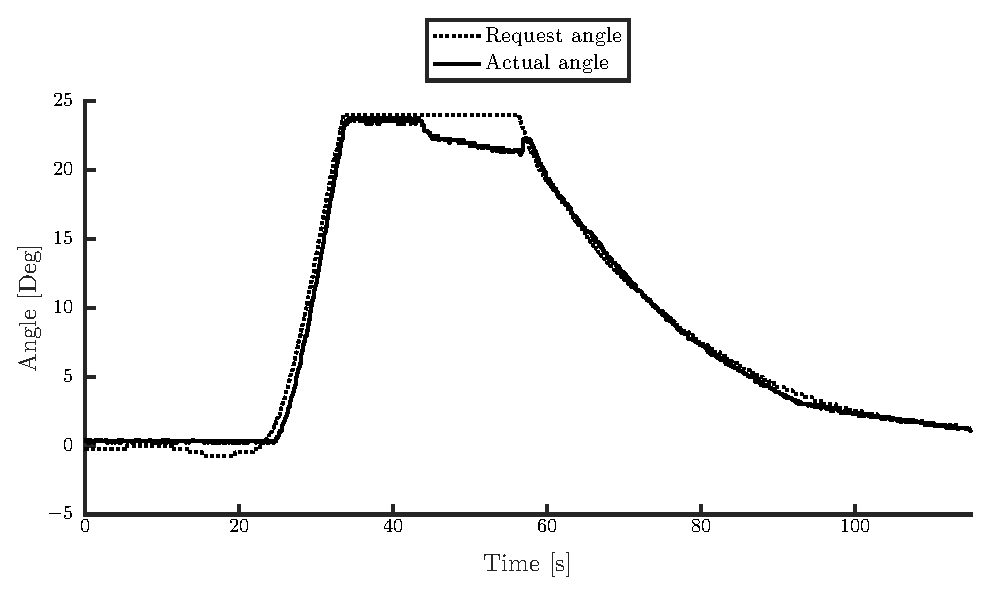
\includegraphics[width=1\linewidth]{front}
		\caption[Decline of steering angles for constant requests]{Decline of steering angles for constant requests}
		
		\label{fig:Constant_request}
	\end{figure}
	
	\begin{figure}[!h]
		
		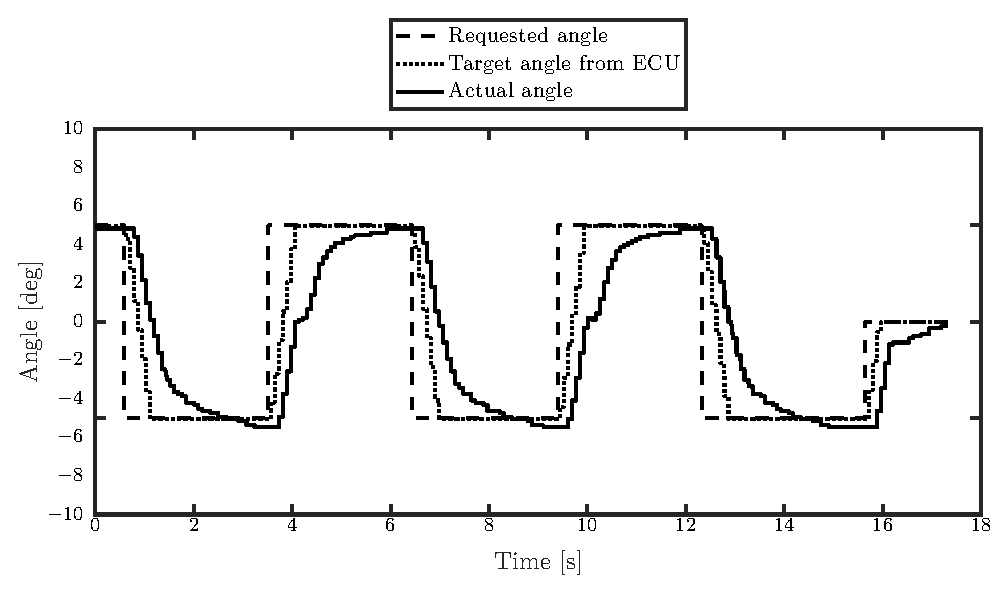
\includegraphics[width=1\linewidth]{Step_input_request}
		\caption[Delay between requested and actual angle]{Delay between requested angle and actual angle}
		
		\label{fig:Step_input_request}
	\end{figure}
	\begin{enumerate}
		\item If a constant steering-angle is requested over a certain period, the hydraulic system will slowly fall back to the middle position. This needs to be eliminated because turning maneuvers or shunting situations often require maximum articulation for longer timespan. Figure \ref{fig:Constant_request} shows this decline, for constant angles.
		
		
		
		\item Around the middle-position the steering does not react towards small changes. The legacy system has a dead band for articulations between +/-2 degrees. For the original application this is useful to ensure a straight path of the vehicle. For this experimental platform however consistent control over the complete range is desirable. This is to also enable small articulations of the axles which is especially called for at higher speeds, where steering angles are a lot smaller. 
		
		\item The steering system has a response time, composed of the normal inertias of the hydraulic system and an additional delay introduced by filtering and noise-canceling in the legacy system. This delays can be gathered from figure \ref{fig:Step_input_request}.
		
		
		
	\end{enumerate}
\begin{figure}[h!]
	
	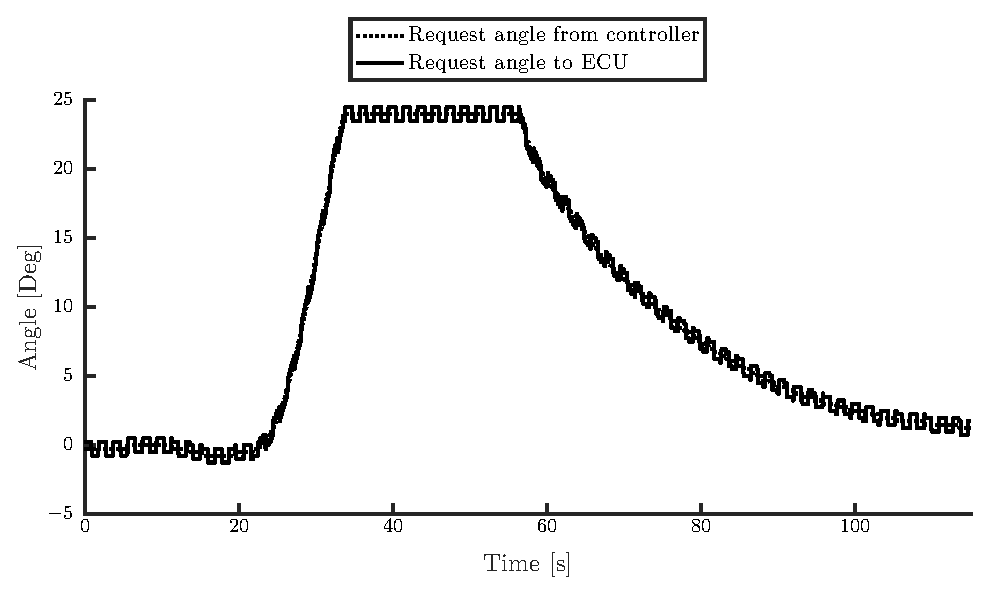
\includegraphics[width=1\linewidth]{Request_with_pulse}
	\caption[Adding a pulsating function to the original request to feed forward to the ECU]{Adding a pulsating function to the original request to feed forward to the ECU}
	\label{fig:Request_with_pulse}
\end{figure}	
	
	Measures to address these issues were:
	
	\begin{enumerate}

		\item To avoid the decline for constant requests, a periodic rectangular function with a small amplitude was added to the requested value and then fed forward to the \gls{ECU}. This is shown in figure \ref{fig:Request_with_pulse}. 
		
		

	\begin{figure}[h!]
		\centering
		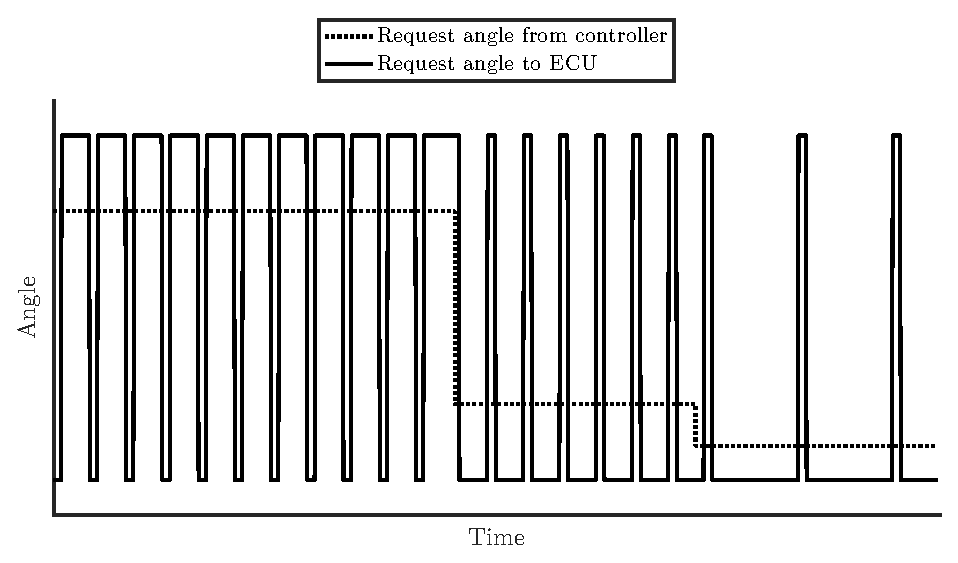
\includegraphics[width=1\linewidth]{Deadband}
		\caption[Sketch of working princiiple of the implemnted PWM to circumvent dead band]{Sketch of working principle of the implemnted PWM to circumvent dead band}
		\label{fig:Deadband}
	\end{figure}
	
		\item A \gls{PWM} around the zero-articulation position reaching out of the dead-band was implemented for requested angles lying within this range. 
		
		
		
		Figure \ref{fig:Deadband} shows the working principle of this measure. The mean value of the request to the \gls{ECU} equals the desired request from the steering algorithm. The pulse function oscilates between specified amplitudes outside the dead band. Through the inertia in the hydraulic system smaller angles can be accomplished, too.
				
		\item Exactly determining the delay period made it possible to account for it in the calculations for initial testing, where a feedback-loop was not present and the speed was still sufficiently low. A value of 0.26\unit{s} for the front axle's reaction time and 0.30\unit{s} for the back axle's respectively are too high for higher speeds.\\
		The introduced noise shown in figure \ref{fig:Request_with_pulse} around the desired request value was also implemented in order to keep the hydraulic system active and thus eliminating some of the inertia. 
	\end{enumerate}
	
	
	
	
	
	
\end{document}